        	\begin{question}{1204}{Vecteurs}{1}{1220}
            	Soient deux vecteurs dans l'espace à 2 dimensions $\vec{A}=(1;1)$ et $\vec{B}=(3;3)$. Quelles sont les coordonnées de $\vec{A}+\vec{B}$?
            \end{question}
            \begin{reponses}
            	\item[false] $(-2;-2)$
            	\item[false] $(2;2)$
                \item[true] $(4;4)$
                \item[false] $(0;0)$
            \end{reponses}
			%%%%%%%%%%%%%%%%%%%%%%%%%%%%%%%%%%%%%
            \begin{question}{1204}{Vecteurs}{2}{1220}
                Quelles sont les coordonnées du vecteur $\vec{AB}+\vec{CD}$?
                \begin{center}
                	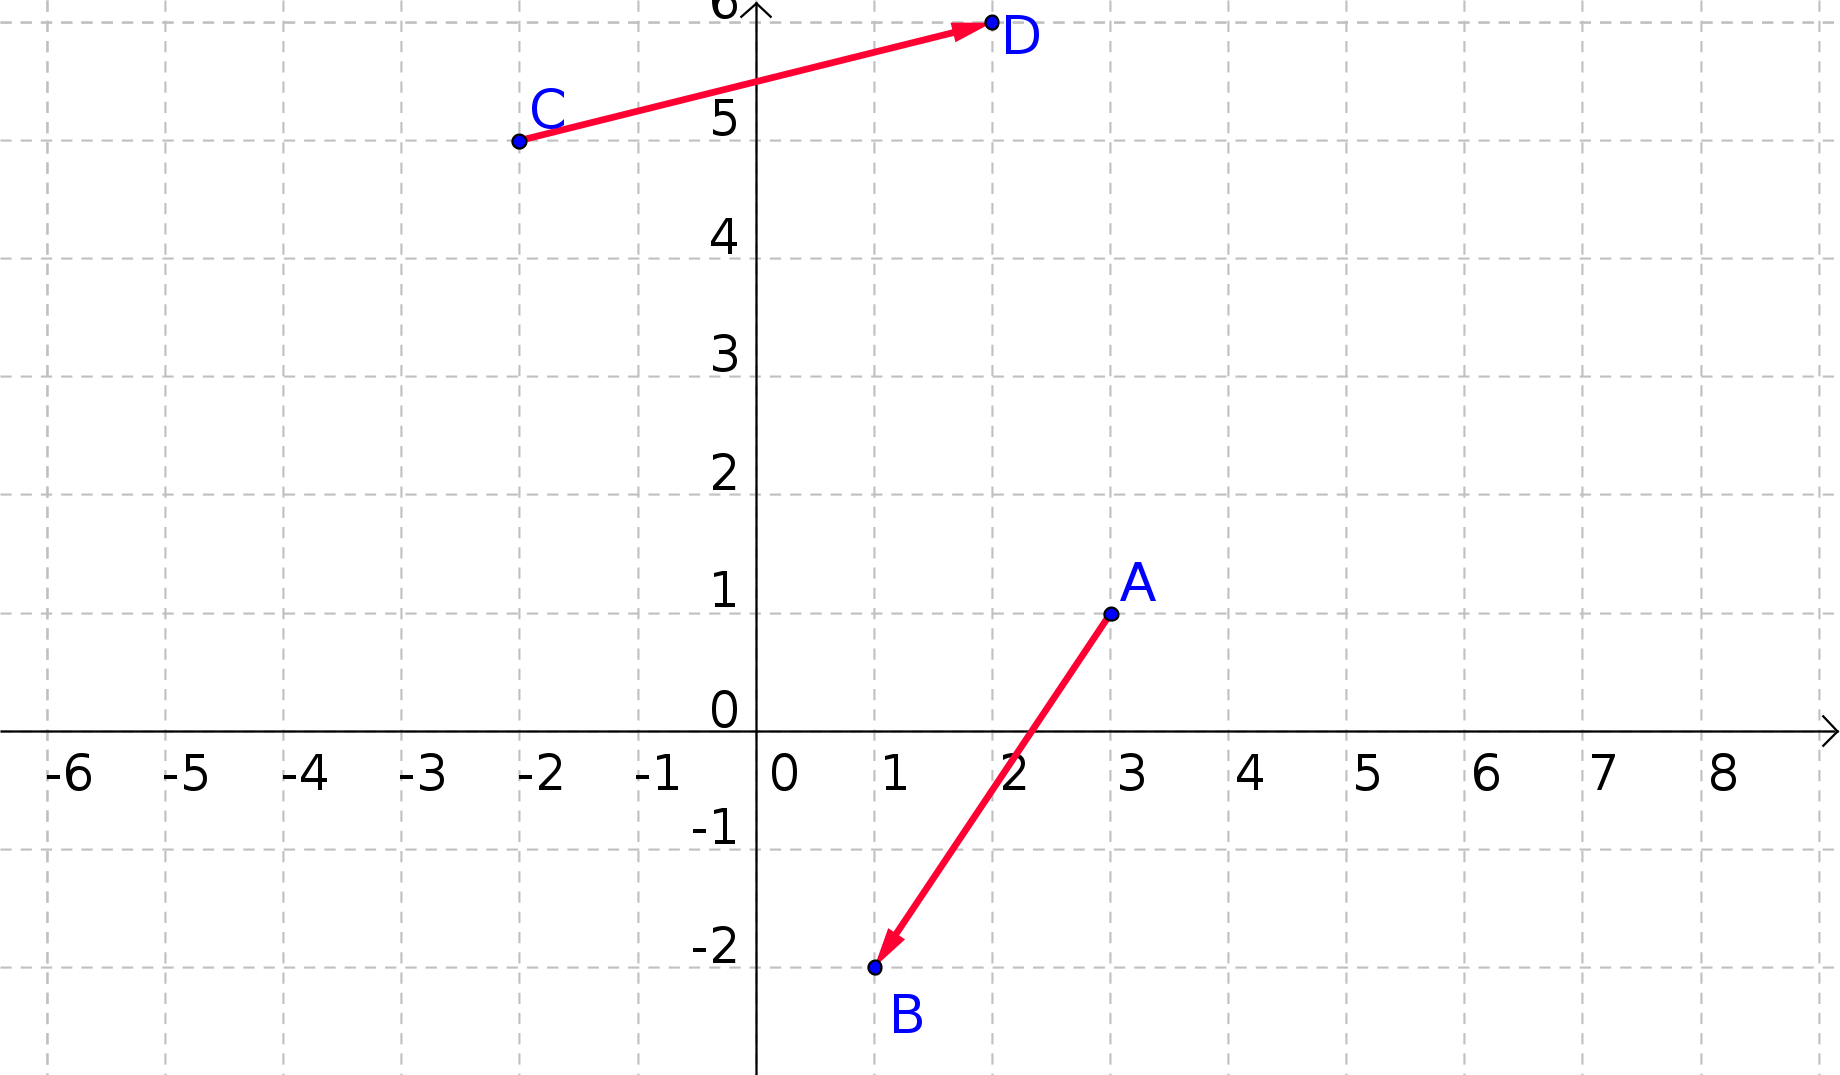
\includegraphics[width=0.5\textwidth]{Philippe/Figures_Philippe/vecteurs_4_4.png}
                \end{center}
            \end{question}
            \begin{reponses}
                \item[false] $(5;7)$
                \item[true] $(2;-2)$
                \item[false] $(-1;-7)$
                \item[false] $(6;4)$
            \end{reponses}
            %%%%%%%%%%%%%%%%%%%%%%%%%%%%%%%%%%%%%
            \begin{question}{1204}{Vecteurs}{2}{1220}
               Soient deux vecteurs de l'espace à 3 dimensions $\vec{A}=(4;2;-2)$ et $\vec{B}=(2;6;1)$. Quelles sont les coordonnées de $\vec{B}-\vec{A}$?
            \end{question}
            \begin{reponses}
                \item[false] $(2;-4;-3)$
                \item[false] $(8;12;2)$
                \item[false] $(-8;-12;-2)$
                \item[true] $(-2;4;3)$
            \end{reponses}
            %%%%%%%%%%%%%%%%%%%%%%%%%%%%%%%%%%%%%
            \begin{question}{1204}{Vecteurs}{2}{1220}
                On sait que la somme des forces extérieures s'appliquant à un objet est égale à la masse multipliée par l'accélération de cet objet. Une masse de \SI{1}{\kilo\gram} subit une force $\vec{F_1}=(0;1;2)$ et une force $\vec{F_2}=(-2;4;-5)$ (en Newton). Que vaut son accélération en \si{\meter\per\second\squared}?
            \end{question}
            \begin{reponses}
                \item[false] $(2;-3;7)$
                \item[false] $(2;-3;3)$
                \item[false] $(-1;-2;5)$
                \item[true] $(-2;5;-3)$
            \end{reponses}
            %%%%%%%%%%%%%%%%%%%%%%%%%%%%%%%%%%%%%
